\chapter{Oscillators}
Three oscillators form the basis of sound generation in Odin 2. You can choose from a wide variety of different modules, which are capable of wide palette of sounds, even without any further processing. Initially, Odin 2 starts out with an Analog Osc in slot 1 and none in slot 2 \& 3. You can change the module being used with the small dropdown button on the top-right of the osc-module:
\vspace{5mm}

\noindent
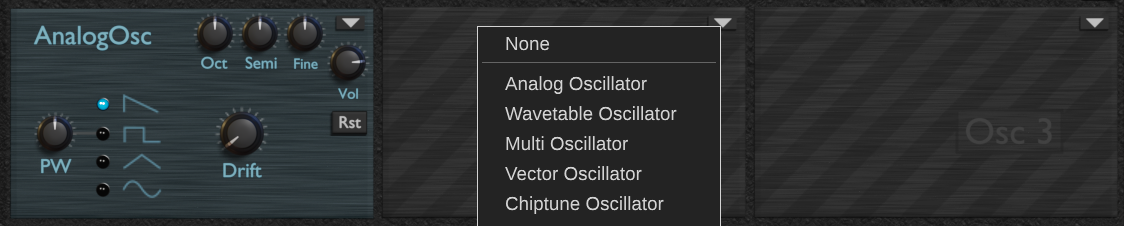
\includegraphics[width=\textwidth]{graphics/osc_selection.png}

\section{Common Parameters}
There are some controls which are common to all oscillator modules:

\audioparameterint{Osc Octave}
Detunes the oscillator by whole octaves.

\audioparameter{Osc Semitones}
Detunes the oscillator by semitones.

\audioparameter{Osc Finetune}
Detunes the oscillator by cents.

\audioparameter{Osc Volume}
Regulates the volume of this oscillator in deciBels. Can be used to shut the oscillator entirely. Modulating this parameter from the \modmatrix  works

